\documentclass[twocolumn]{IEEEtran}
\usepackage[utf8]{inputenc}
\usepackage{graphicx}
\graphicspath{{figs/}} % No modificar
\usepackage{float}
\usepackage{listings}
\usepackage{xcolor}
\usepackage{multicol}
\lstset{
    basicstyle=\ttfamily\scriptsize,
    breaklines=true,
    breakatwhitespace=false,
    columns=fullflexible,
    frame=single,
    numbers=left,
    numbersep=4pt,
    numberstyle=\tiny,
    xleftmargin=1.5em,
    tabsize=2,
    keywordstyle=\color{blue},
    commentstyle=\color{gray},
    stringstyle=\color{teal}
}
\usepackage[spanish, es-tabla]{babel} % Configura el idioma a español
\addto\captionsspanish{\renewcommand{\abstractname}{Abstract}}

\addto\captionsspanish{\renewcommand{\figurename}{Figura}}
\addto\captionsspanish{\renewcommand{\tablename}{Tabla}}
\usepackage{subcaption}
\usepackage{hyperref}
\hypersetup{
    colorlinks=true,
    linkcolor=blue, % Cambia el color del número si lo deseas
    urlcolor=blue,
}

% \usepackage{ulem}
% http://ctan.org/pkg/{algorithms,algorithmx}
% \usepackage{algorithms,algorithmx}
\renewcommand{\thetable}{\arabic{table}}

\usepackage{hyperref}
\hypersetup{
    colorlinks=true,
    linkcolor=blue,
    filecolor=magenta,      
    urlcolor=blue,
    citecolor = blue,
}
\usepackage{tikz}

\newcommand{\hilight}[1]{\colorbox{yellow}{#1}}
%\numberwithin{equation}{section}
\usepackage{booktabs}
\usepackage{xcolor}
\usepackage{multirow}
\newtheorem{theorem}{Theorem}[section]
\makeatletter
\newcommand{\settheoremtag}[1]{% \settheoremtag{<tag>}
  \let\oldthetheorem\thetheorem% Store \thetheorem
  \renewcommand{\thetheorem}{#1}% Redefine it to a fixed value
  \g@addto@macro\endtheorem{% At \end{theorem}, ...
    \addtocounter{theorem}{-1}% ...restore theorem counter value and...
    \global\let\thetheorem\oldthetheorem}% ...restore \thetheorem
  }
\usepackage{titlesec}

% Cambiar tamaño de las secciones
\titleformat{\section}
  {\normalsize\bfseries}   % tamaño y estilo (large = un poco más grande que normal)
  {\thesection}{1em}  % numeración
  {}

\titleformat{\subsection}
  {\normalsize\bfseries} % tamaño de subsección
  {\thesubsection}{1em}
  {}

% PASO 1. Reemplace "Práctica 1" por el número de la práctica que corresponda
\newcommand{\dochead}{Práctica #1)}     

% PASO 2. Verifique el título de la práctica corresponda.
\newcommand{\docsubhead}{Introducción a GNURadio, python block y GitHub}  

% PASO 3. Reemplace "B1A - 02" por el grupo de la asignatura y el número de su grupo de laboratorio
\newcommand{\teamname}{A1-E}     

% PASO 4. OPCIONAL: Reemplace "\docsubhead \docsubhead" por el título del documento en caso de requerirse.
\newcommand{\titulo}{\dochead: \docsubhead}      

% PASO 5. Reemplace "31 de diciembre de 2030" por la fecha de su documento
\newcommand{\fecha}{Agosto 27, 2026}     

\input{./plantilla.tex}             % No modificar

\usepackage{titlesec}
\titlespacing*{\section}
{0pt}{1ex}{1ex}  % Ajusta el espacio antes y después de las secciones

\usepackage[hidelinks]{hyperref}
\begin{document}  

% No modificar

\title{\vspace{1cm}\textbf{\titulo}}            % No modificar

% PASO 6. Agregar aquí el nombre y código de los autores.  
\author{
Jarol Nicolas Molano Lopez - 2230391 \\
William Camilo Motta Chacon - 2234639\\
Juan Andres Rojas Rueda - 2231065
}
\affil{\small{\url{https://github.com/J202R/2026_2_ComII_A1_A1E}}}
\affil{\normalsize{Escuela de Ingenierías Eléctrica, Electrónica y de Telecomunicaciones} \\ % No modificar
\small{Universidad Industrial de Santander}} % No modificar

\date{\today}

\maketitle                          % No modificar
\thispagestyle{fancy}               % No modificar

%---------------------------------------------------------------
% PASO 7. **..**...****INICIE SU DOCUMENTO DESDE AQUI***...**...
%%%%% A PARTIR DE AQUÍ EDITE EL DOCUMENTO PARA AGREGAR TODO EL CONTENIDO REQUERIDO PARA EL ENTREGABLE CORRESPONDIENTE
%%%%  Todo el contenido a partir de este punto es SOLAMENTE ILUSTRATIVO.
%
% Para sus imformes, BORRE TODO el contenido de aquí en adelante  EXCEPTO la última línea que contiene el comando: \end{document}




% \begin{multicols}{2}
\begin{abstract}
This document presents the design and implementation of custom blocks for real-time signal processing in Software Defined Radio (SDR) systems. Discrete accumulation, differentiation, and statistical analysis algorithms applied to continuous signals are evaluated. Finally, a practical application focused on noise characterization and mitigation in real environments is validated through the integration of the developed modules.
\end{abstract}
 
 






\begin{IEEEkeywords}
GNURadio,Python block
\end{IEEEkeywords}

\section{Introducción}

El procesamiento digital de señales en tiempo real requiere la implementación e integración de operaciones matemáticas y algorítmicas capaces de manipular flujos continuos de datos. En el estudio de los sistemas de radiocomunicaciones y la radio definida por software (SDR), resulta indispensable ir más allá de los módulos funcionales predefinidos y desarrollar bloques de código personalizados que permitan ejecutar tareas específicas de procesamiento, acondicionamiento y análisis de señales.

Esta práctica de laboratorio se enfoca en el diseño, implementación y evaluación de bloques de procesamiento programados a medida. Específicamente, se abordan operaciones fundamentales en el dominio discreto como la acumulación, la diferenciación temporal y el cálculo de parámetros estadísticos sobre señales continuas. Finalmente, estos módulos se integran en una aplicación práctica orientada a la caracterización y mitigación de ruido en señales reales, evaluando el desempeño de los algoritmos implementados frente a perturbaciones estocásticas.








\section{Metodología}

Se implementaron y modificaron los bloques personalizados en Python (\textit{Embedded Python Block} \cite{wikipediaPythonBlocks}) propuestos por el libro guía\cite{ortega2019comunicaciones} 
en GNU Radio Companion, correspondientes a un acumulador y un diferenciador, 
operaciones inversas entre sí que sirven de base para el análisis estadístico 
posterior.

\subsection{Bloque acumulador}
El código base obtenido de \cite{ortega2019comunicaciones} reiniciaba la suma en cada bloque de datos (\textit{buffer}), 
generando discontinuidades, y retornaba \texttt{len(y)}, variable inexistente. 
Se corrigió agregando una variable de estado (\texttt{valor\_anterior}) que 
conserva el último valor entre llamados a \texttt{work}, y se corrigió el retorno 
a \texttt{len(y0)}.

\begin{lstlisting}[caption={Bloque acumulador con memoria de estado}, label={lst:acumulador}]
import numpy as np
from gnuradio import gr
class blk(gr.sync_block):
    def __init__(self):
        gr.sync_block.__init__(
            self, name='e_Acum',
            in_sig=[np.float32],
            out_sig=[np.float32])
        self.valor_anterior = 0.0
    def work(self, input_items, output_items):
        x = input_items[0]
        y0 = output_items[0]
        y0[:] = self.valor_anterior + np.cumsum(x)
        if len(y0) > 0:
            self.valor_anterior = y0[-1]
        return len(y0)
\end{lstlisting}

\subsection{Bloque diferenciador}


El código base \cite{ortega2019comunicaciones}  tenía un error de sintaxis (asignación fuera del constructor sin 
cerrar paréntesis) y no conservaba la última muestra entre buffers, afectando la 
primera diferencia de cada bloque. Se corrigió la sintaxis y se añadió la variable 
\texttt{muestra\_anterior}, insertada al inicio del vector de entrada antes de 
aplicar \texttt{np.diff}.

\begin{lstlisting}[caption={Bloque diferenciador con continuidad entre buffers}, label={lst:diferenciador}]
import numpy as np
from gnuradio import gr
class blk(gr.sync_block):
    def __init__(self):
        gr.sync_block.__init__(
            self, name='e_Diff',
            in_sig=[np.float32],
            out_sig=[np.float32])
        self.muestra_anterior = 0.0
    def work(self, input_items, output_items):
        x = input_items[0]
        y0 = output_items[0]
        if len(x) == 0:
            return 0
        x_completo = np.insert(
            x, 0, self.muestra_anterior)
        y0[:] = np.diff(x_completo)
        self.muestra_anterior = x[-1]
        return len(y0)
\end{lstlisting}

\subsection{Bloque de estadísticas de tiempo}

A partir de los bloques anteriores y el libro guía \cite{ortega2019comunicaciones} 
se implementó un bloque adicional que calcula, de forma acumulativa, cinco 
estimadores estadísticos: media, media cuadrática (MS), RMS, potencia promedio y 
desviación estándar.

El código base presentaba un error en el cálculo de la media cuadrática, ya que al 
actualizar \texttt{acum\_anterior1} se referenciaba por error el vector 
\texttt{acumulado} (de la media) en lugar de \texttt{acumulado1}, invalidando dicho 
cálculo. Además, el bloque devolvía vectores completos por cada muestra procesada, 
cuando solo interesa el valor global acumulado.

Se corrigió el error de referencia y se simplificó el cálculo utilizando 
acumuladores escalares (\texttt{acum\_x}, \texttt{acum\_x2}), calculando media y 
media cuadrática de forma directa. La desviación estándar se obtuvo a partir de la 
identidad $\sigma^2 = E[X^2] - (E[X])^2$, en lugar de acumular residuales al 
cuadrado, reduciendo la complejidad del bloque y evitando una tercera variable de 
estado. Se incluyó además una validación para evitar valores negativos de varianza 
por errores de precisión numérica.


\begin{figure}[t]
\centering
\begin{minipage}[t]{0.48\linewidth}
\begin{lstlisting}[basicstyle=\tiny\ttfamily, firstnumber=1]
import numpy as np
from gnuradio import gr
class blk(gr.sync_block):
    def __init__(self):
        gr.sync_block.__init__(
            self, name='
              Promedios_de_tiempos
            ',
            in_sig=[np.float32],
            out_sig=[np.float32]*5
        )
        self.acum_x = 0.0
        self.acum_x2 = 0.0
        self.Ntotales = 0
    def work(self, input_items,
             output_items):
        x = input_items[0]
        y0, y1, y2, y3, y4 = \
            output_items
        N = len(x)
\end{lstlisting}
\end{minipage}
\hfill
\begin{minipage}[t]{0.48\linewidth}
\begin{lstlisting}[basicstyle=\tiny\ttfamily, firstnumber=21]
        if N == 0:
            return 0
        self.Ntotales += N
        self.acum_x += np.sum(x)
        self.acum_x2 += np.sum(x**2)
        media = self.acum_x / self.
            Ntotales
        ms = self.acum_x2 / self.
            Ntotales
        rms = np.sqrt(ms)
        var = ms - media**2
        if var < 0:
            var = 0
        std = np.sqrt(var)
        y0[:] = media
        y1[:] = ms
        y2[:] = rms
        y3[:] = ms
        y4[:] = std
        return len(x)
\end{lstlisting}
\end{minipage}
\caption*{\textbf{Listing 3:} Bloque de estadísticas de tiempo}
\label{lst:estadisticas}
\end{figure}














\subsection{Aplicación: análisis estadístico de una señal ECG}

Como aplicación de los bloques implementados, se utilizó una señal real de ECG 
limpia, correspondiente al registro 118 de la base de datos MIT-BIH Arrhythmia 
Database \cite{moody2005mitdb}. A esta señal se le añadió ruido gaussiano 
artificial mediante un bloque \textit{Noise Source} y un bloque \textit{Add}, el 
cual fue posteriormente atenuado con un bloque \textit{Moving Average} como se explicó en \cite{tijaro2025timeaverages}, las configuraciones de este bloque correspondieron a una de longitud 
4 muestras y una escala de $1/M$ para realizar correctamente los promedios temporales y cumplir con la frecuencia máxima $f_{max}=40$ Hz.


\begin{equation}
    \hat{\omega}_{max} = \frac{2\pi f_{max}}{f_s} \leq \frac{\pi}{N} \implies N \leq \frac{f_s}{2 f_{max}} = \frac{360}{2 \times 40} = 4.5
\end{equation}

Cabe aclarar que la ecuación aplicada fue extraída de \cite{wavewalkerdsp2022ma}, la frecuencia de muestreo fue determinada desde el repositorio y la $f_{max}$ establecida por convención para monitoreo clínico. Las tres versiones de la señal (original, con ruido y filtrada) se 
conectaron a tres instancias del bloque \textit{Promedios\_de\_tiempos}, con el fin 
de comparar sus estimadores estadísticos y evaluar el efecto del ruido y del 
filtrado sobre ellos.



\section{RESULTADOS Y ANÁLISIS DE DATOS}

Para validar el funcionamiento de los bloques implementados se diseñaron dos 
esquemas de prueba en GNU Radio Companion, uno para el diferenciador y otro para 
el acumulador, utilizando bloques \textit{Vector Source} con señales conocidas y 
bloques \textit{QT GUI Time Sink} para visualizar simultáneamente la señal de 
entrada y la señal de salida de cada proceso.

\subsection{Prueba del bloque diferenciador}

Como se observa en la figura \ref{fig:diff_test}, al ingresar una señal constante 
de valor 5.5 al bloque \textit{e\_Diff}, la señal de salida permanece en cero a lo 
largo de todo el tiempo de observación, ya que al no existir variación entre 
muestras consecutivas la diferencia calculada  es 
siempre nula. Por otro lado, al ingresar la señal periódica tipo rampa con el 
patrón $1,2,3,4,5,0$, se observa que la salida del diferenciador presenta saltos 
correspondientes a las diferencias entre valores consecutivos del patrón 
($1,1,1,1,-5$), repitiéndose de forma periódica junto con la señal de entrada. 
Este comportamiento evidencia que el bloque responde únicamente a los cambios de 
la señal y no a su magnitud absoluta, validando el funcionamiento esperado del 
algoritmo implementado.

\begin{figure}[!ht]
    \centering
    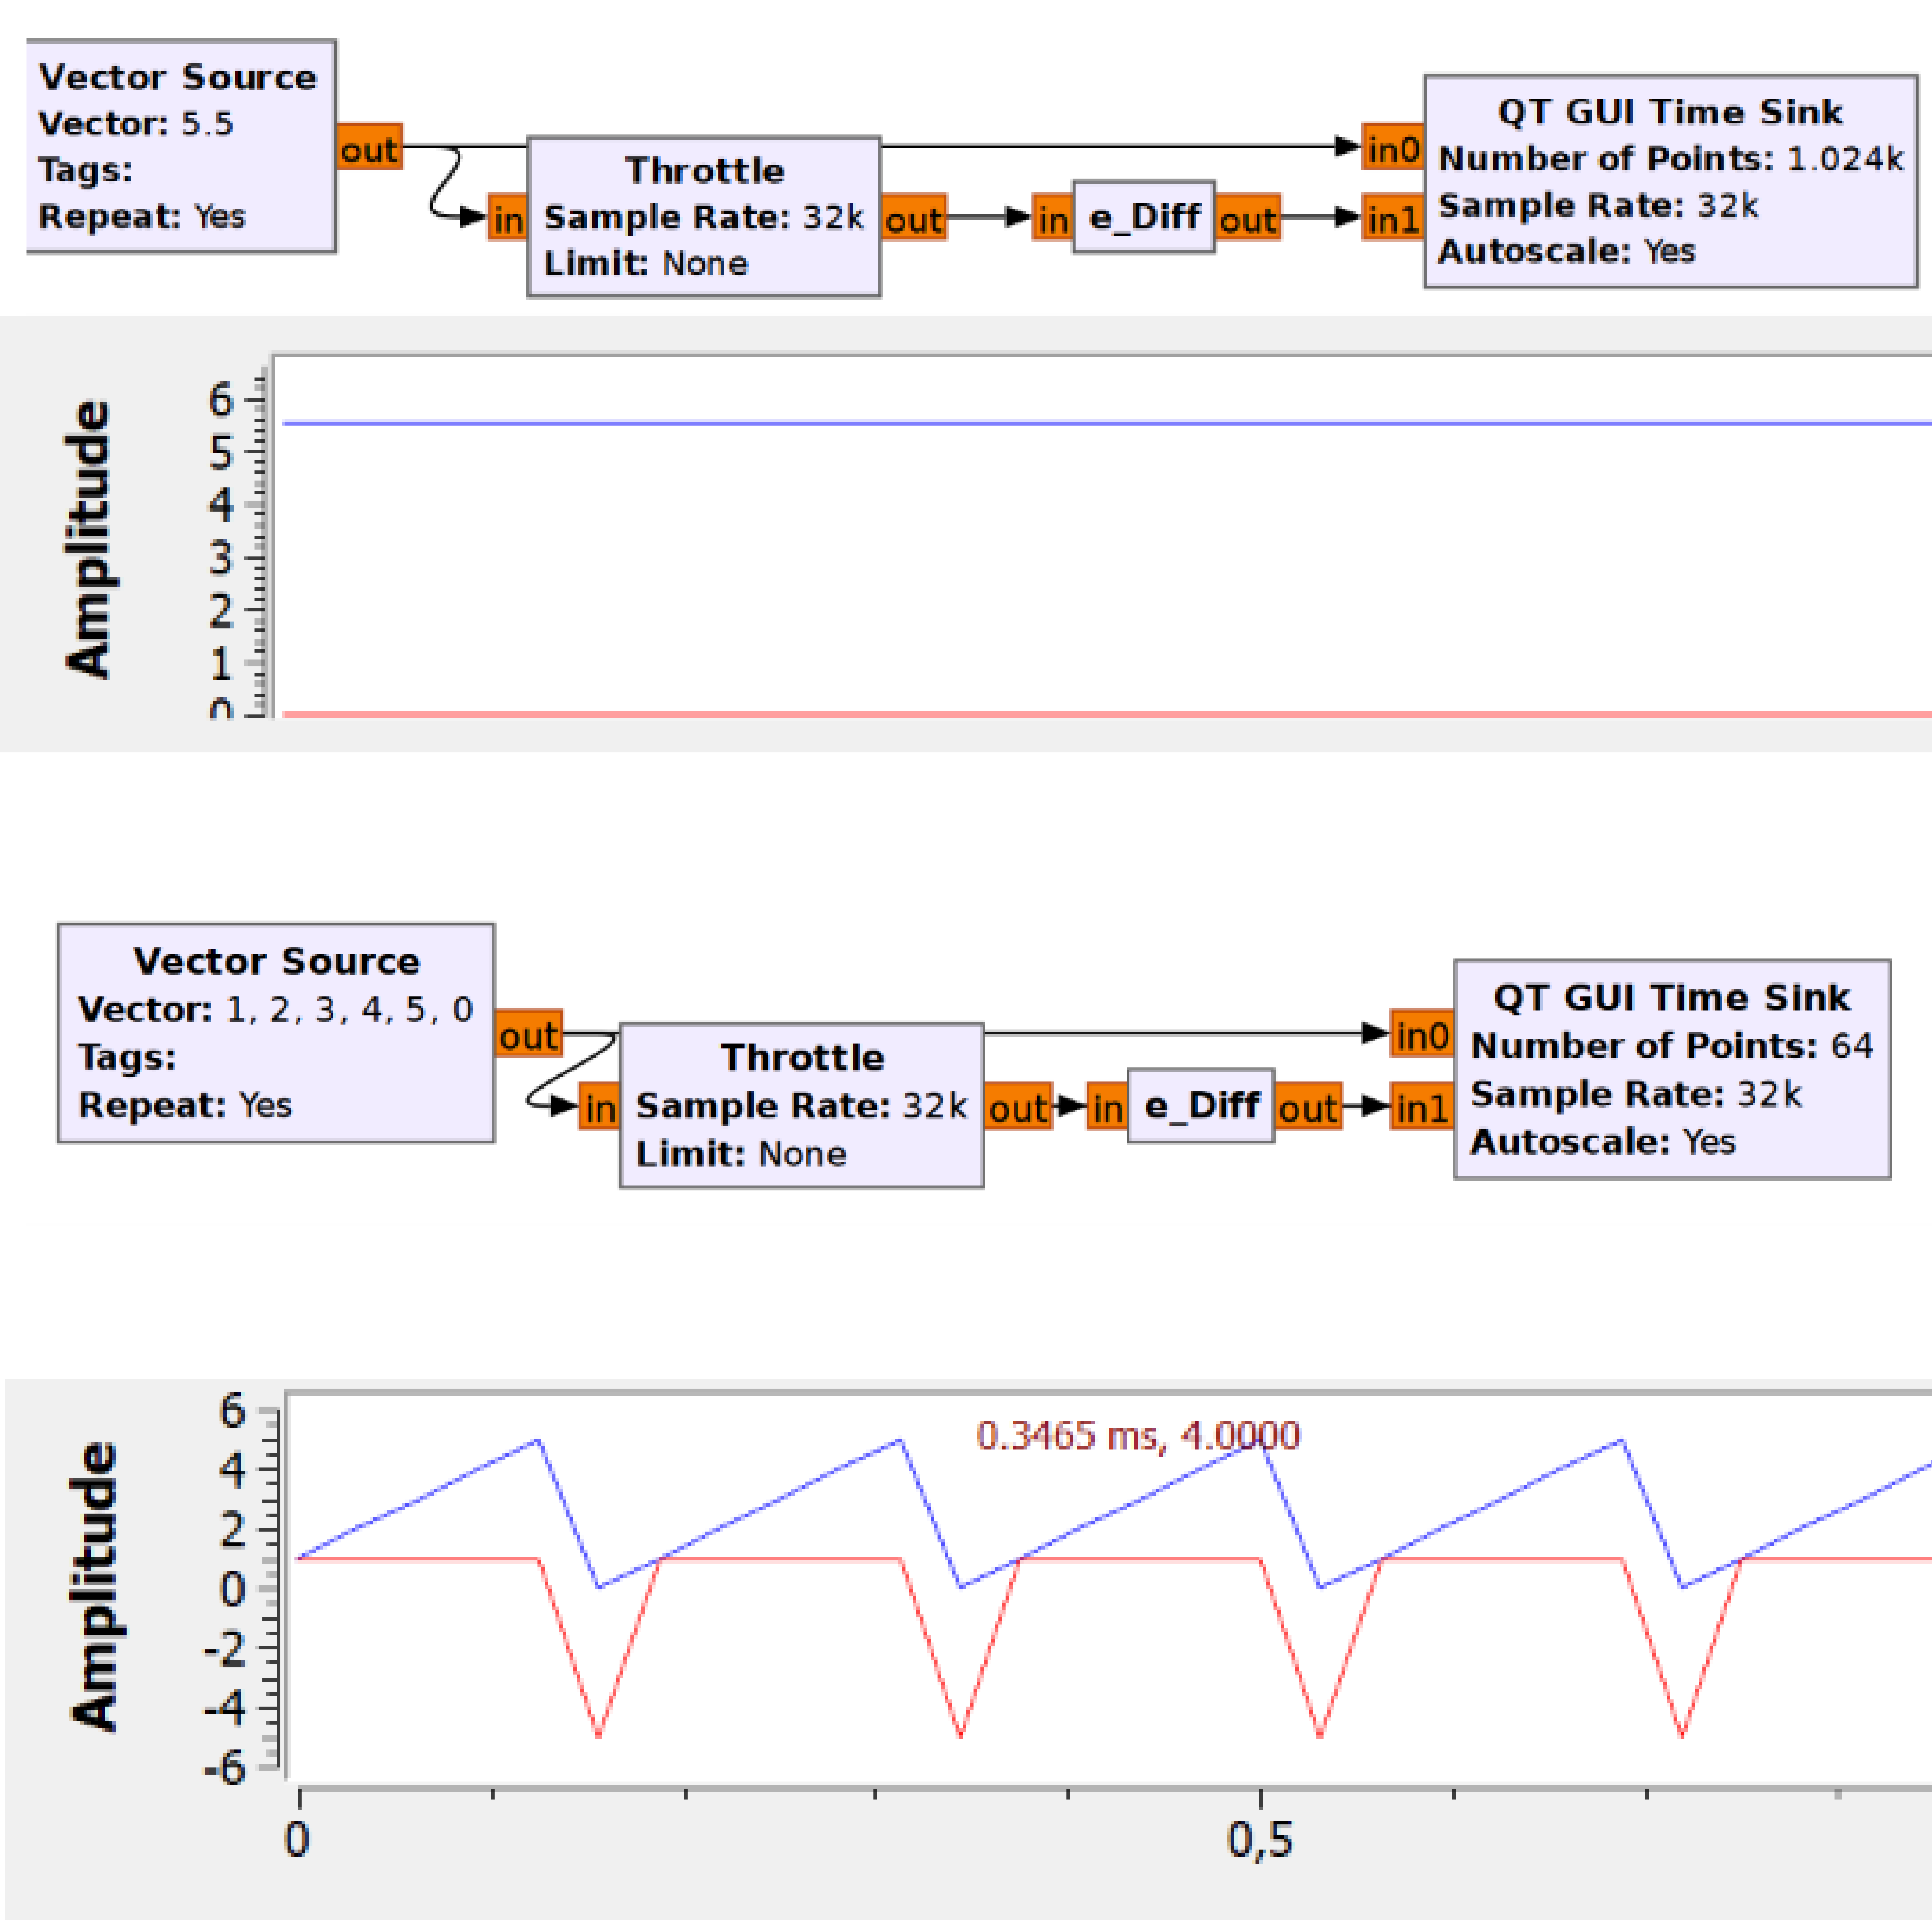
\includegraphics[width=0.8\linewidth]{imagenes/diferenciador_resultado.pdf}
    \caption{Diagrama de bloques y resultado de la prueba del bloque diferenciador para dos señales de entrada: una señal constante de valor 5.5 y una señal periódica tipo rampa con el patrón 1,2,3,4,5,0.}
    \label{fig:diff_test}
\end{figure}
\subsection{Prueba del bloque acumulador}

Como se observa en la figura \ref{fig:acum_test}, al ingresar una señal constante 
de valor $1\text{m}$ al bloque \textit{e\_Acum}, la señal de salida crece de forma 
lineal en el tiempo, generando una rampa cuya pendiente corresponde al valor de la 
señal de entrada, tal como lo predice la teoría. Se observa, 
además que dicho crecimiento se mantiene continuo a lo largo de todo el registro, 
sin saltos ni reinicios entre los distintos bloques de procesamiento, lo cual 
confirma que el estado interno del bloque (\texttt{valor\_anterior}) conserva 
correctamente la acumulación entre llamados sucesivos a la función \texttt{work}.

\begin{figure}[!ht]
    \centering
    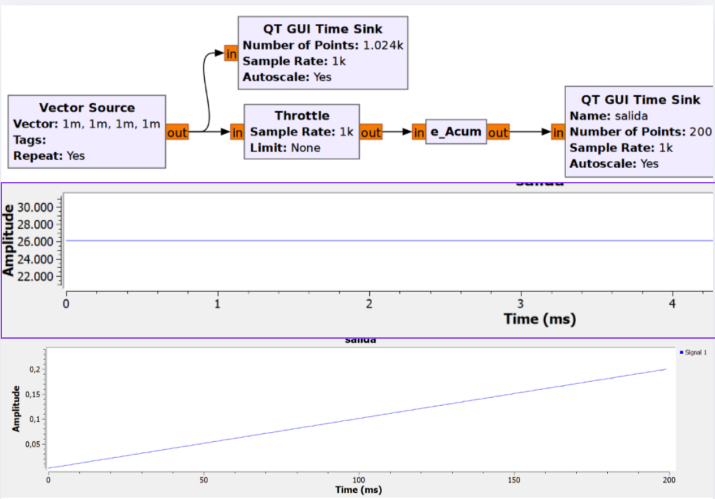
\includegraphics[width=0.8\linewidth]{imagenes/acumulador_resultado.png}
    \caption{Diagrama de bloques y resultado de la prueba del bloque acumulador para una señal de entrada constante de valor 1m, mostrando el crecimiento lineal (tipo rampa) generado en la señal de salida.}
    \label{fig:acum_test}
\end{figure}






\subsection{Prueba del bloque de estadísticas de tiempo}

Como se observa en la figura \ref{fig:estadisticas_test}, el bloque 
\textit{Promedios\_de\_tiempos} se alimentó con una señal cosenoidal de frecuencia 
1 kHz, amplitud 1 y frecuencia de muestreo 32 kHz, obteniendo simultáneamente los 
cinco estimadores estadísticos a través de bloques \textit{QT GUI Number Sink}. 
Dado que la señal tiene media nula, la \textit{Media} converge a un valor cercano 
a cero, mientras que la \textit{Media cuadrática} y la \textit{Potencia promedio} 
convergen a $0.5$, consistente con la potencia teórica de una cosenoidal de 
amplitud unitaria ($A^2/2$). En consecuencia, el \textit{RMS} se aproxima a 
$0.707$ ($1/\sqrt{2}$), y la \textit{Desviación estándar} converge a un valor 
similar al RMS, confirmando que los estimadores implementados corresponden a sus 
definiciones teóricas.

\begin{figure}[!ht]
    \centering
    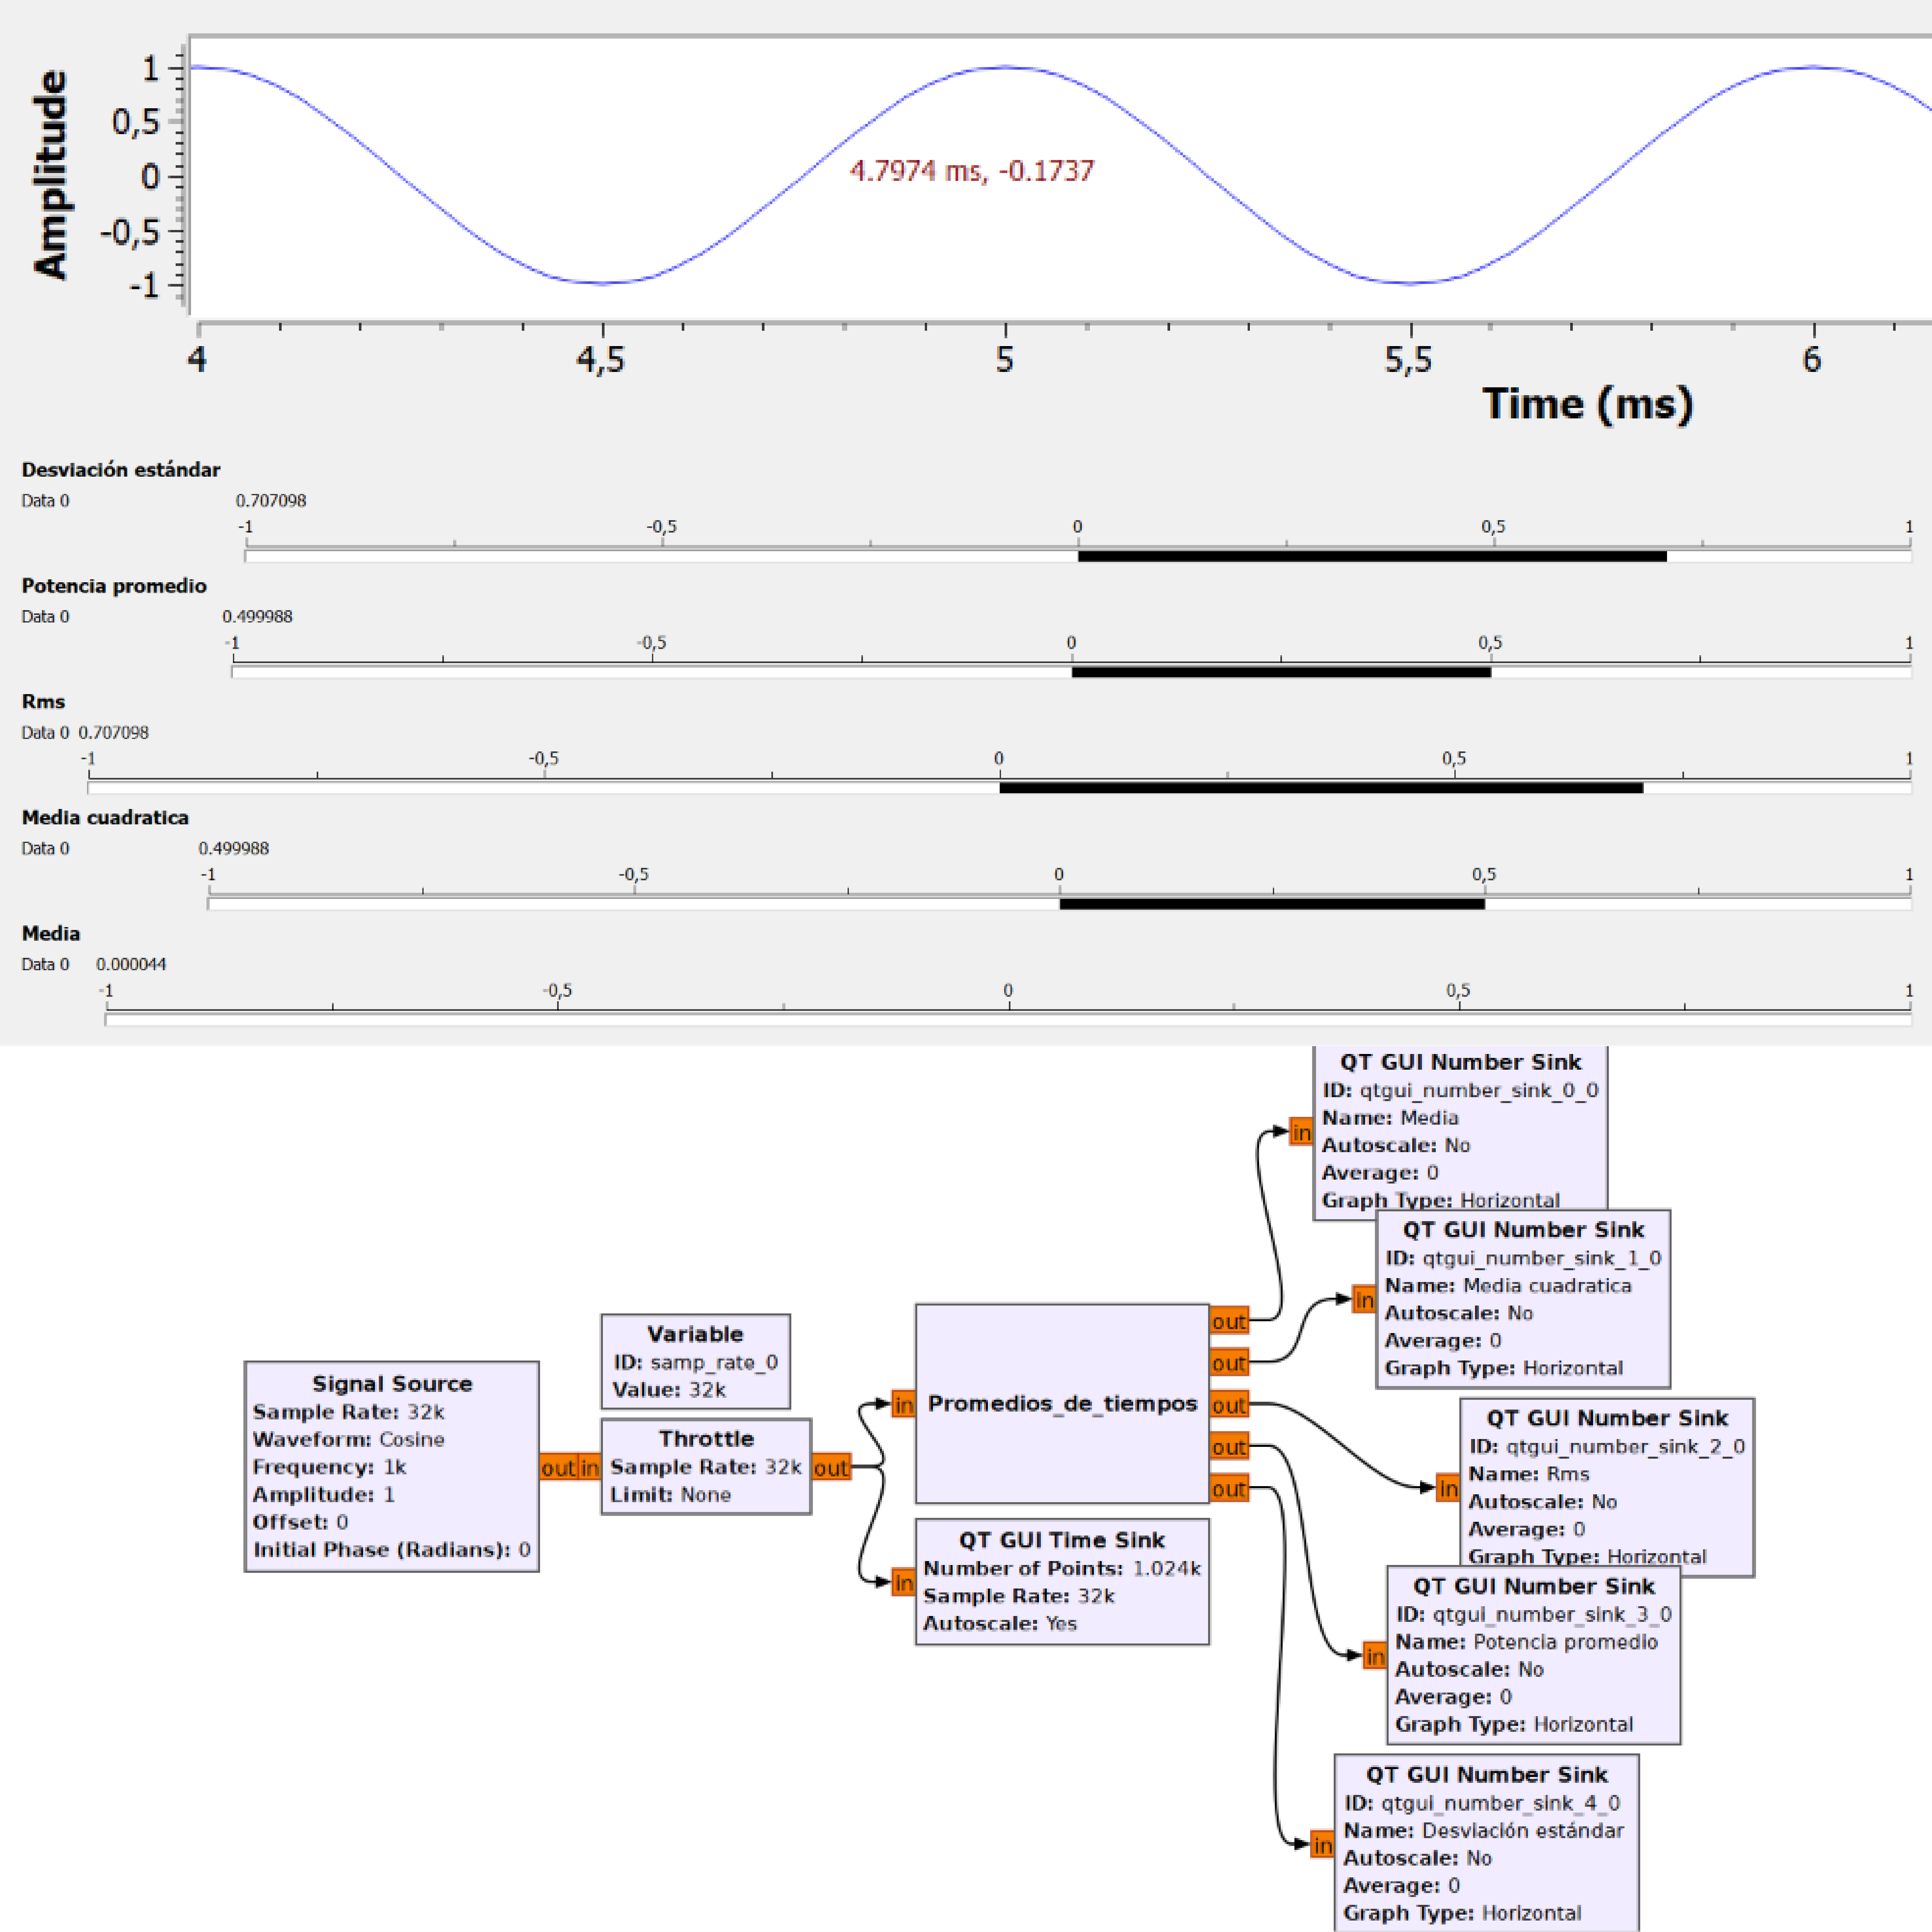
\includegraphics[width=0.8\linewidth]{imagenes/estadisticas_resultado}
    \caption{Diagrama de bloques y resultados del bloque de estadísticas de tiempo para una señal cosenoidal de 1 kHz, amplitud 1 y frecuencia de muestreo de 32 kHz: media, media cuadrática, RMS, potencia promedio y desviación estándar.}
    \label{fig:estadisticas_test}
\end{figure}











\subsection{Prueba de la aplicación con señal ECG}

En la figura \ref{fig:ecg_test} se presenta el esquema implementado, donde la 
señal original, la señal con ruido añadido y la señal filtrada usando moving average \cite{tijaro2025timeaverages} se procesan 
simultáneamente. La tabla \ref{tab:ecg_stats} resume los estimadores obtenidos 
para cada caso.

\begin{figure}[!ht]
    \centering
    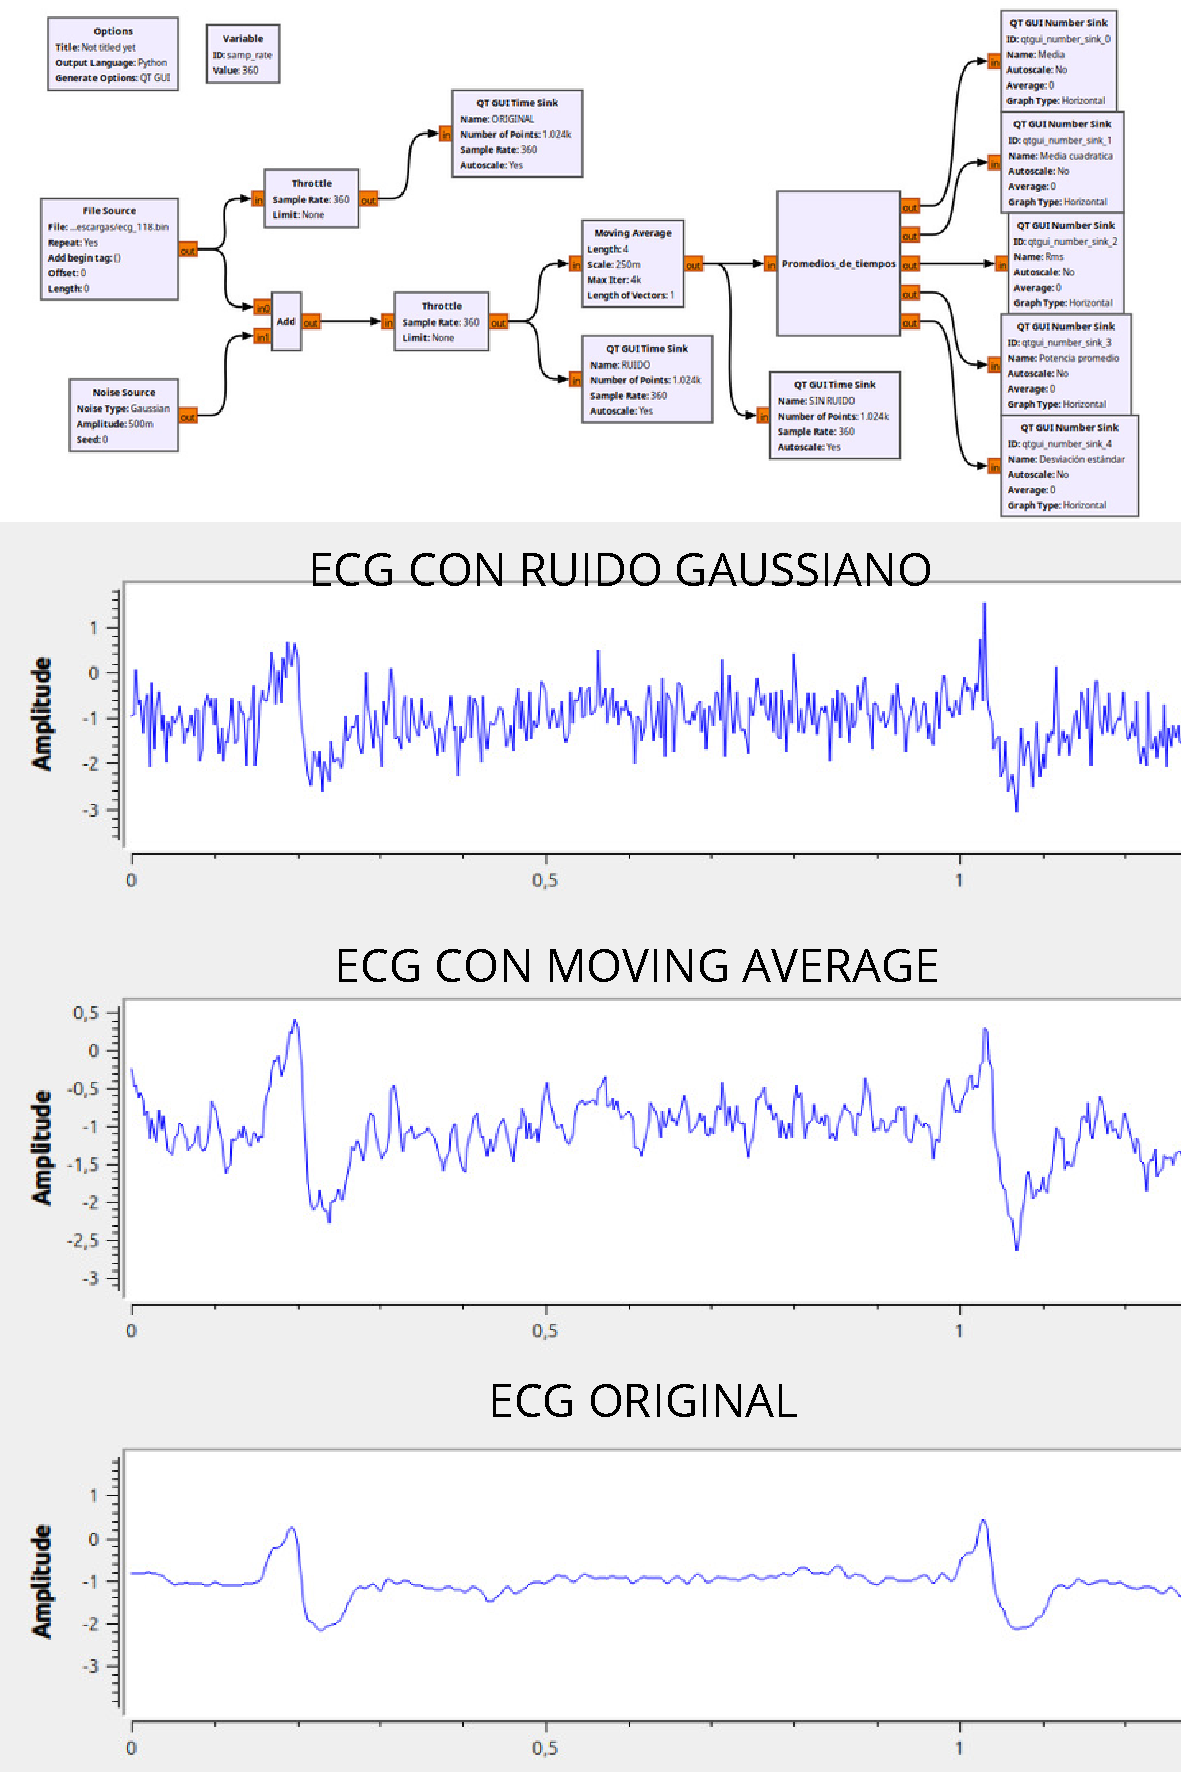
\includegraphics[width=0.65\linewidth]{imagenes/ecg_resultado}
    \caption{Esquema de la aplicación del bloque de estadísticas sobre una señal ECG del registro 118 de la base MIT-BIH \cite{moody2005mitdb} : señal original, con ruido gaussiano añadido y filtrada mediante promedio móvil.}
    \label{fig:ecg_test}
\end{figure}



\begin{table}[!ht]
    \centering
    \caption{Comparación de estimadores estadísticos para la señal ECG original, con ruido añadido y filtrada}
    \label{tab:ecg_stats}
    \begin{tabular}{lccc}
        \hline
        \textbf{Estimador} & \textbf{Original} & \textbf{Con ruido} & \textbf{Filtrada} \\
        \hline
        Desviación estándar & 0.404398  & 0.638660  & 0.439031 \\
        Potencia promedio   & 1.176480  & 1.412420  & 1.241412
 \\
        RMS                 & 1.084656  & 1.188453  & 1.114187
\\
        Media cuadrática    & 1.176480  & 1.412420  & 1.241412
 \\
        Media               & -1.006450 & -1.002264 & -1.024043\\
        \hline
    \end{tabular}
\end{table}

De los valores recopilados en la tabla \ref{tab:ecg_stats} se identifica que la señal con ruido añadido presenta valores más altos que los de la señal 
original, dado que el ruido gaussiano tiene amplitud de (500m) frente a la 
señal ECG, aumentando levemente la mayoría de estimadores excepto la media que redujo ligeramente su valor. En 
cambio, la señal filtrada presenta cambios menos notorios y mucho más cercanos a los de la señal original,
lo cual indica que el \textit{Moving Average} no solo atenúa el ruido, sino que 
también modifica la forma de la señal al promediar sus muestras, por lo que su 
efecto sobre los estimadores debe interpretarse con cuidado.

























\section{Conclusiones}
Se identificaron los aspectos fundamentales del procesamiento en tiempo real, respecto al bloque acumulador (código~\ref{lst:acumulador}), la variable de 
estado \texttt{valor\_anterior} permitió conservar la acumulación entre buffers, 
eliminando los reinicios de la versión original. Esto se confirma en la 
figura \ref{fig:acum_test}, donde una entrada constante de 1m genera una rampa 
lineal y continua en la salida, sin saltos entre llamados a \texttt{work}, 
validando el correcto funcionamiento del bloque \textit{e\_Acum} como operación 
inversa del diferenciador.
Como se observa en la figura \ref{fig:diff_test}, el 
diferenciador respondió correctamente ante la señal de entrada constante en la cual se observó el comportamiento adecuado, dando como resultado una salida con valor cero, de igual manera, para la rampa se presentó la salida correcta. De igual forma, en la figura 
\ref{fig:estadisticas_test} los estimadores estadísticos calculados convergieron 
a los valores teóricos esperados para una señal cosenoidal.


    Finalmente, la aplicación sobre la señal ECG (figura~\ref{fig:ecg_test}, 
tabla~\ref{tab:ecg_stats}) permitió evidenciar cuantitativamente el efecto del 
ruido y del filtrado sobre los estimadores estadísticos: la señal ruidosa 
presentó los valores más altos de desviación estándar, potencia promedio y RMS, 
mientras que el filtrado con \textit{Moving Average} redujo dichos valores 
acercándolos a los de la señal original, aunque sin recuperarlos por completo, 
debido a la modificación de la forma de onda introducida por el promedio móvil. 
Esto confirma la utilidad práctica del bloque \textit{Promedios\_de\_tiempos} 
como herramienta de caracterización de señales antes y después de un proceso de 
filtrado.

% NO MODIFIQUE NI ELIMINE ESTA PARTE PARA QUE APAREZCAN LAS REFERENCIAS



\nocite{*}

\bibliographystyle{IEEEtran}
\bibliography{bibliografia}

\end{document}